Antes de profundizar en los detalles del funcionamiento del prototipo, es fundamental presentar su estructura lógica general.
\\
\\
El prototipo está centrado exclusivamente en la entidad usuario, quien es el único actor que interactúa directamente con el sistema. Una vez que accede a la plataforma, el usuario puede visualizar y participar en diversas lecciones, las cuales están compuestas por un conjunto de preguntas.
\\
\\
Cada lección se organiza de forma estructurada, incluyendo un texto base que introduce el tema de la lección, seguido de dos preguntas. Cada pregunta está acompañada por su respuesta correcta y una incorrecta, lo cual permite evaluar la comprensión del usuario.

\section{Diseño de base de datos}
\noindent La base de datos relacional para el prototipo tiene como objetivo central gestionar la información relacionada con los usuarios y su proceso de aprendizaje a través de lecciones y preguntas (dicho proceso se explica a mas detalle en el capitulo 6). Para ello, se estructura en seis (6) tablas principales: \textbf{usuarios}, \textbf{lecciones}, \textbf{preguntas}, \textbf{registro\_preguntas}, \textbf{lecciones\_resueltas} y \textbf{rachas}. Cada una de estas tablas cumple una función específica dentro del sistema y se encuentra relacionada para facilitar el acceso eficiente y coherente a los datos.
\\
\\
A continuación se presenta una descripción breve de cada tabla:
\begin{itemize}
  \item \textbf{usuarios}: almacena la información principal de cada usuario del sistema.
  \item \textbf{lecciones}: contiene los registros de las lecciones generadas, incluyendo su contenido.
  \item \textbf{preguntas}: guarda el contenido de las preguntas asociadas a cada lección.
  \item \textbf{registro\_preguntas}: almacena el resultado de las preguntas que el usuario ha respondido, permitiendo realizar un seguimiento de las preguntas respondidas incorrectamente para reutilizarlas en la sección de preguntas incorrectas del prototipo.
  \item \textbf{lecciones\_resueltas}: registra todas las lecciones que el usuario ya ha completado.
  \item \textbf{rachas}: controla elementos de gamificación, como la cantidad de días consecutivos en los que un usuario ha respondido correctamente al menos una pregunta y la experiencia global obtenida.
\end{itemize}

\subsection{Modelo Entidad Relación }

\begin{figure}[H]
  \centering
  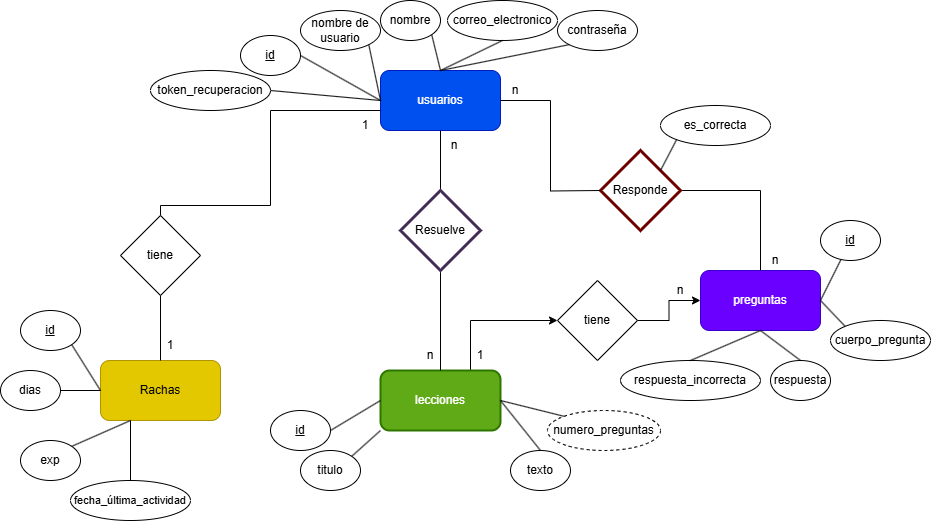
\includegraphics[width=0.9\linewidth]{Imagenes/DB_RM.png}
  \caption{Modelo Entidad Relación}
  \label{fig:ER}
\end{figure}


\subsection{Modelo UML}

\begin{figure}[H]
  \centering
  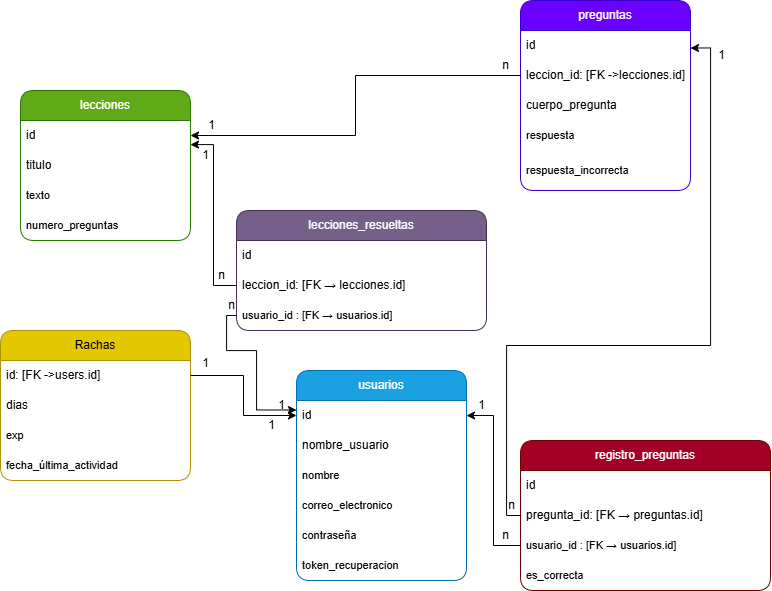
\includegraphics[width=0.6\linewidth]{Imagenes/DB_UML.png}
  \caption{Modelo UML}
  \label{fig:uml}
\end{figure}


\subsection{Base de datos NoSQL}

A diferencia de las bases de datos relacionales, Redis, al ser una base de datos NoSQL (Not Only SQL) no utiliza un esquema estructurado predefinido, ya que se basa en el almacenamiento de datos en formato clave-valor. Por esta razón, a continuación se detalla las claves utilizadas, los tipos de datos asociados y una breve descripción de su propósito dentro del sistema. Esta representación permite comprender la lógica de almacenamiento empleada en Redis y su papel en el prototipo.

\begin{table}[H]
\centering
\begin{tabular}{|p{3.5cm}|l|p{6cm}|}
\hline
\textbf{Tipo} & \textbf{Nombre de la variable} & \textbf{Descripci\'on} \\
\hline
Hash & \texttt{lesson:\{lesson\_id\}} & Almacena atributos de la lecci\'on: ID, t\'itulo y cantidad de preguntas. Esto con el objetivo de brindar en la pagina principal del prototipo una breve descripcion de todas las lecciones recientes. \\
\hline
Conjunto (set) & \texttt{all\_lessons} & Contiene todas las claves de lecciones creadas recientemente. Se utiliza para acceder a todas las lecciones actuales de forma eficiente. \\
\hline
Conjunto (set) & \texttt{user:\{user\_id\}:completed} & Guarda los ID de las lecciones completadas por un usuario espec\'ifico. Facilita brindar al usuario solo las lecciones actuales que tiene pendientes por realizar. \\
\hline
\end{tabular}
\caption{Estructuras de datos utilizadas en Redis}
\label{table:EstructurasRedis}
\end{table}
